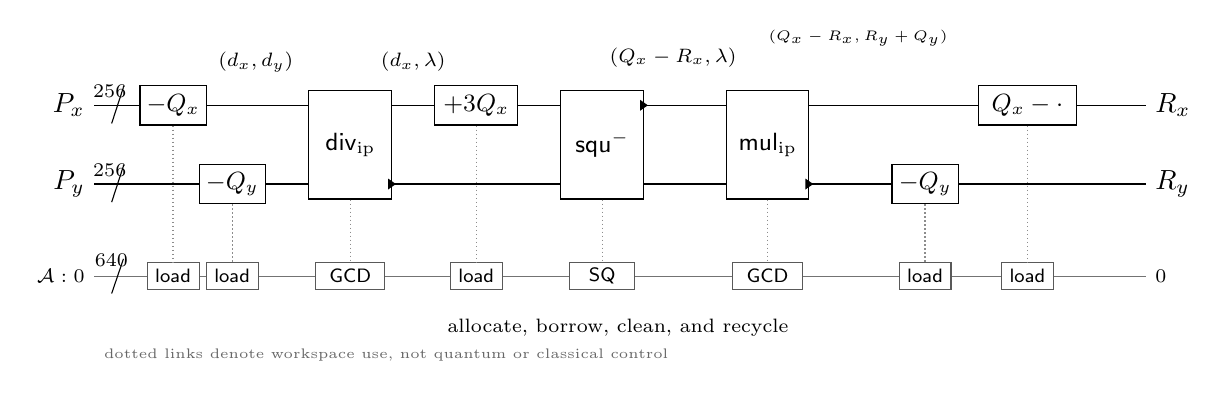
\begin{tikzpicture}[
  x=1cm,
  y=1cm,
  wire/.style={draw=black, line width=0.45pt},
  scratchwire/.style={draw=black!55, line width=0.4pt},
  scratchlink/.style={draw=black!45, densely dotted, line width=0.45pt},
  block/.style={
    draw=black,
    fill=white,
    minimum height=0.50cm,
    minimum width=0.84cm,
    inner sep=2pt,
    font=\small
  },
  wideblock/.style={
    draw=black,
    fill=white,
    minimum height=1.38cm,
    minimum width=1.05cm,
    inner sep=2pt,
    align=center,
    font=\small
  },
  scratchblock/.style={
    draw=black!65,
    fill=white,
    minimum height=0.34cm,
    minimum width=0.48cm,
    inner sep=1pt,
    font=\scriptsize
  },
  state/.style={font=\scriptsize, inner sep=1pt}
]

% The two interface registers and the pooled physical workspace.
\draw[wire] (0,1.35) -- (13.35,1.35);
\draw[wire] (0,0.35) -- (13.35,0.35);
\draw[scratchwire] (0,-0.82) -- (13.35,-0.82);
\node[left] at (0,1.35) {$\ket{P_x}$};
\node[left] at (0,0.35) {$\ket{P_y}$};
\node[left, font=\scriptsize] at (0,-0.82)
  {$\mathcal A:\ket{0}$};
\node[right] at (13.35,1.35) {$\ket{R_x}$};
\node[right] at (13.35,0.35) {$\ket{R_y}$};
\node[right, font=\scriptsize] at (13.35,-0.82) {$\ket{0}$};

% Register-bundle marks.
\draw (0.22,1.12) -- (0.37,1.58);
\node[font=\scriptsize, anchor=east] at (0.53,1.53) {$256$};
\draw (0.22,0.12) -- (0.37,0.58);
\node[font=\scriptsize, anchor=east] at (0.53,0.53) {$256$};
\draw (0.22,-1.04) -- (0.37,-0.60);
\node[font=\scriptsize, anchor=east] at (0.55,-0.62) {$640$};

% Runtime-classical coordinate subtraction.  These are sequential in code
% and share the same allocator pool.
\node[block] (subx) at (1.00,1.35) {$-Q_x$};
\node[scratchblock, minimum width=0.66cm] (subxs) at (1.00,-0.82)
  {$\mathsf{load}$};
\draw[scratchlink] (subx.south) -- (subxs.north);
\node[block] (suby) at (1.75,0.35) {$-Q_y$};
\node[scratchblock, minimum width=0.66cm] (subys) at (1.75,-0.82)
  {$\mathsf{load}$};
\draw[scratchlink] (suby.south) -- (subys.north);
\node[state] at (2.05,1.90) {$(d_x,d_y)$};

% In-place division Y <- Y/X, implemented by forward/reverse GCD walks.
\node[wideblock] (div) at (3.25,0.85)
  {$\mathsf{div}_{\rm ip}$};
\node[scratchblock, minimum width=0.88cm] (divs) at (3.25,-0.82)
  {$\mathsf{GCD}$};
\draw[scratchlink] (div.south) -- (divs.north);
\fill (3.83,0.35) -- (3.73,0.42) -- (3.73,0.28) -- cycle;
\node[state] at (4.05,1.90) {$(d_x,\lambda)$};

% Prepare the output-side x difference.
\node[block, minimum width=1.05cm] (add3) at (4.85,1.35) {$+3Q_x$};
\node[scratchblock, minimum width=0.66cm] (add3s) at (4.85,-0.82)
  {$\mathsf{load}$};
\draw[scratchlink] (add3.south) -- (add3s.north);
\node[wideblock] (squ) at (6.45,0.85) {$\mathsf{squ}^{-}$};
\node[scratchblock, minimum width=0.82cm] (squs) at (6.45,-0.82)
  {$\mathsf{SQ}$};
\draw[scratchlink] (squ.south) -- (squs.north);
\fill (7.03,1.35) -- (6.93,1.42) -- (6.93,1.28) -- cycle;
\node[state] at (7.35,1.96) {$(Q_x-R_x,\lambda)$};

% Convert the slope into the output-side numerator.
\node[wideblock] (mul) at (8.55,0.85)
  {$\mathsf{mul}_{\rm ip}$};
\node[scratchblock, minimum width=0.88cm] (muls) at (8.55,-0.82)
  {$\mathsf{GCD}$};
\draw[scratchlink] (mul.south) -- (muls.north);
\fill (9.13,0.35) -- (9.03,0.42) -- (9.03,0.28) -- cycle;
\node[state, font=\tiny] at (9.70,2.20) {$(Q_x-R_x,R_y+Q_y)$};

% Restore canonical output coordinates.  The reverse subtraction fuses the
% always-on tail -2Qx, +Qx, neg of the controlled construction in Figure 9.
\node[block] (subqy) at (10.55,0.35) {$-Q_y$};
\node[scratchblock, minimum width=0.66cm] (subqys) at (10.55,-0.82)
  {$\mathsf{load}$};
\draw[scratchlink] (subqy.south) -- (subqys.north);
\node[block, minimum width=1.25cm] (rsub) at (11.85,1.35)
  {$Q_x-\mathord{\cdot}$};
\node[scratchblock, minimum width=0.66cm] (rsubs) at (11.85,-0.82)
  {$\mathsf{load}$};
\draw[scratchlink] (rsub.south) -- (rsubs.north);

% Direction of computation and interpretation of the third bus.
\draw[->, line width=0.45pt] (4.95,-1.48) -- (8.35,-1.48);
\node[font=\scriptsize, fill=white, inner sep=1pt] at (6.65,-1.48)
  {allocate, borrow, clean, and recycle};
\node[font=\tiny, text=black!60, anchor=west] at (0,-1.82)
  {dotted links denote workspace use, not quantum or classical control};

\end{tikzpicture}
